\newpage
\chapter{Design Changes}
\label{chap:design_changes}
% what major design changes have been introduced since the CDR report? Argument why these changes were necessary. Also, will be good to include test results (functionality, weight, performance etc.) which are not documented in the CDR report.
%
%
\section{Project Schedule, Resources and Goals}
\label{sec:project_changes}
%responsible: Morten
%
As previously stated in [CDR ref], the U-SPACE project was initially substantially delayed due to bureaucratic challenges in course registrations and subsequent release of project budget. This resulted in a reformulation of the system concept going from a custom designed helium envelope to a \ac{COTS} blimp provided by Esrange Space Center.

In June 2012, many of the U-SPACE team members left Kiruna to pursue summer internships and prepare for their 3rd semester outside Sweden. Work on the project over the summer holiday was restricted since Lars Jakobsson (LTU technician) was unavailable thus making ordering of new components impossible. Work on U-SPACE began again in September 2012, when Jan and Pedro returned to Sweden and Omair officially joined the project. At this point, Morten took over the full project management responsibilities and also remained responsible for the power subsystem, Jan became the lead responsible for the attitude sensors and payload, Omair responsible for all on-board telemetry handling, telecommunication and ground station and Pedro responsible for the mechanical structure and motors.

Since the sun sits very low on the horizon during autumn in Kiruna and is almost completely absent during winter, it was decided, for the first prototype, not to implement the solar array and related electronics. Instead the goal would be to realize an indoor battery powered flight. This also reduced the work load as was required due to the fewer people now working on the project.

Weekly status meetings were held with project supervisors, but internal meetings were only held on a need-basis since the group just counted four people and were often already sitting together in the Viking project room. 
Due to some misunderstandings of the initial budget, it was approved by the supervisors to increase the project budget for the four remaining students from 2000 SEK to 2500 SEK per student. 


\section{Electrical Power Subsystem}
%responsible: Morten
%
Due to the issues discussed in section \ref{sec:project_changes}, the solar cells were not ordered. However, it is still believed that the cells discussed in [ref to CDR] are suitable for this project.
%
%
In the final circuity layouts, it was decided to place the \ac{BCR} and \ac{SAR} on separate \acp{PCB}. Additionally, a small temperature sensor board was built. The following sections describe the features and circuit diagrams of each of these boards.
%
%
\subsection{Battery}
%
%Challenges in thermal design to achieve specifications on battery. A passive design has been made. Specify test results. Suggestion to add a heater or have a winter + summer configuration of the insulation.
%
During testing of a thermal design, one Li-ion battery underwent a heavy discharge and subsequently showed clear indication of damage (swallowing of the battery pack). There was no immediate danger, however the incidence learned us that it is important that everyone working with Li-ion batteries knows about its safe use and limitations. Li-ion fires are almost impossible to put out. Only useful method is to cover the battery in sand why we recommend LTU to put available a bucket of sand and/or establish a fire proof area/table for working with Li-ion batteries.
%
%
\subsection{Battery Charge Regulator}
%
Table \ref{tab:BCR_features} lists the features of the final \ac{BCR}.
%
\begin{table}[H]
\centering
\caption{Features of developed \ac{BCR}}
\label{tab:BCR_features}
\begin{tabular}{p{0.35\textwidth}p{0.2\textwidth}p{0.4\textwidth}}
\hline
\textbf{Feature/Specification} & \textbf{Value} & \textbf{Comments}\\
\hline
Max output current & 20 A & All outputs combined \\
Output voltage & 6-8 V & Unregulated \\
Input voltage & 9.2-9.5 V & Higher voltage may lead to overheating\\
Weight & ??? & \\
Under voltage protection & $V_{BATT}$ < 6.0 V & Only cuts off motor power outputs \\
Short-circuit protection & $I_{SC}$ > 15 A & Only on motor power outputs \\
Thermal monitoring and charge cut-off & & \\
Automatic charge control & - & Constant current or voltage and trickle charge\\
Charge inhibit by telecommand & & \\
Power cut-off by telecommand & & Only motor power outputs\\
Charge status telemetry & &\\
Charge/discharge current monitoring & & \\
Battery cells voltage monitoring & & \\
\hline
\end{tabular}
\end{table} 
%
The main changes to the \ac{BCR} include added telemetries, telecommands and protection circuits.
%
%
\subsubsection*{Increasing BCR Power Output}
The chosen Li-ion battery can supply up to 66 A continuously or 88 A burst. The main limitation of the \ac{BCR} power output is due to current ratings on the power diode (20 A), power connectors (19 A) and wires (19 A or 11.5 A when using ECSS derating[ref to ECSS]). PCB trace thickness may also become impractically thick at higher currents. 
To increase the output power rating, the best and first option is to use a higher battery voltage by connecting several batteries in series (or using a higher voltage battery pack with more cells in series). 
The current rating can also be increased by using higher power connectors, thicker wire or several wires in parallel, higher power diodes or two diodes in parallel and using thicker PCB copper tracing, reducing trace length, increasing trace width and improving the thermal layout (adding lots of heat sinks and thermal connections).
%
%
All \ac{BCR} functionalities have been tested and verified at room temperature conditions.
%
\begin{figure}[H]
\begin{minipage}[t]{\linewidth}
\centering
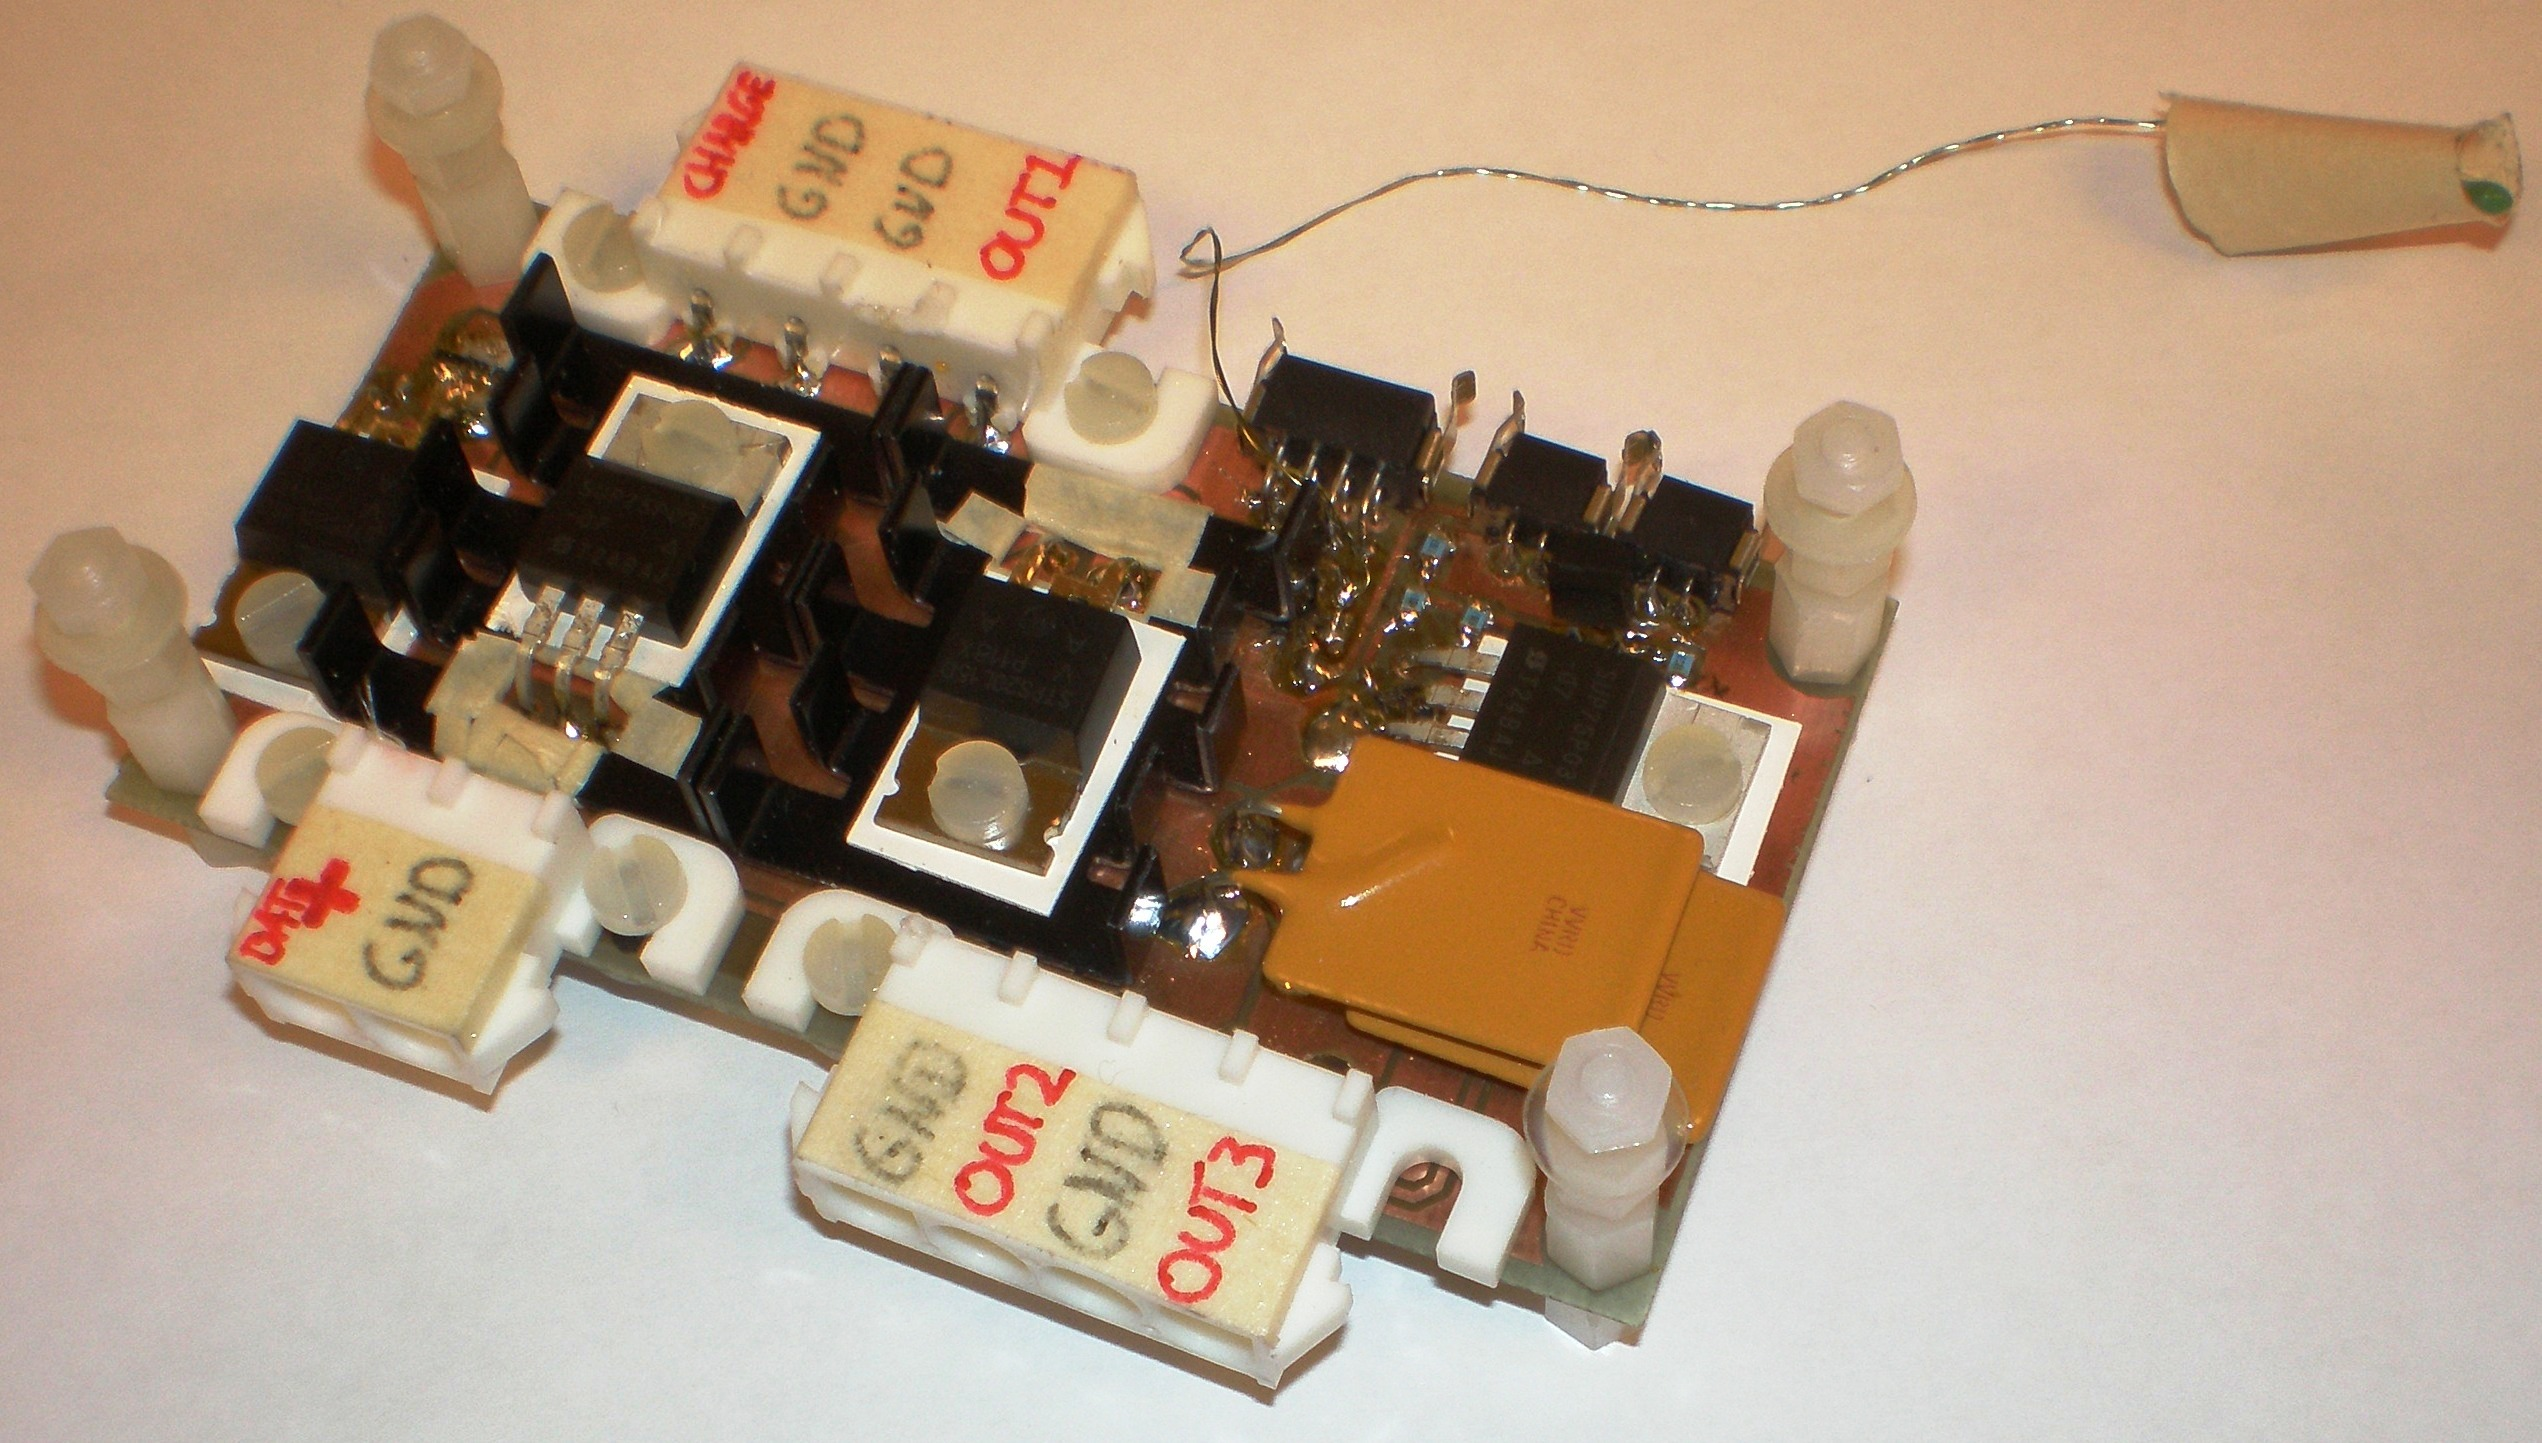
\includegraphics[width=0.7\textwidth]{figures/fig_BCR_top}
\end{minipage}
\vspace{2mm}
\begin{minipage}[t]{\linewidth}
\centering
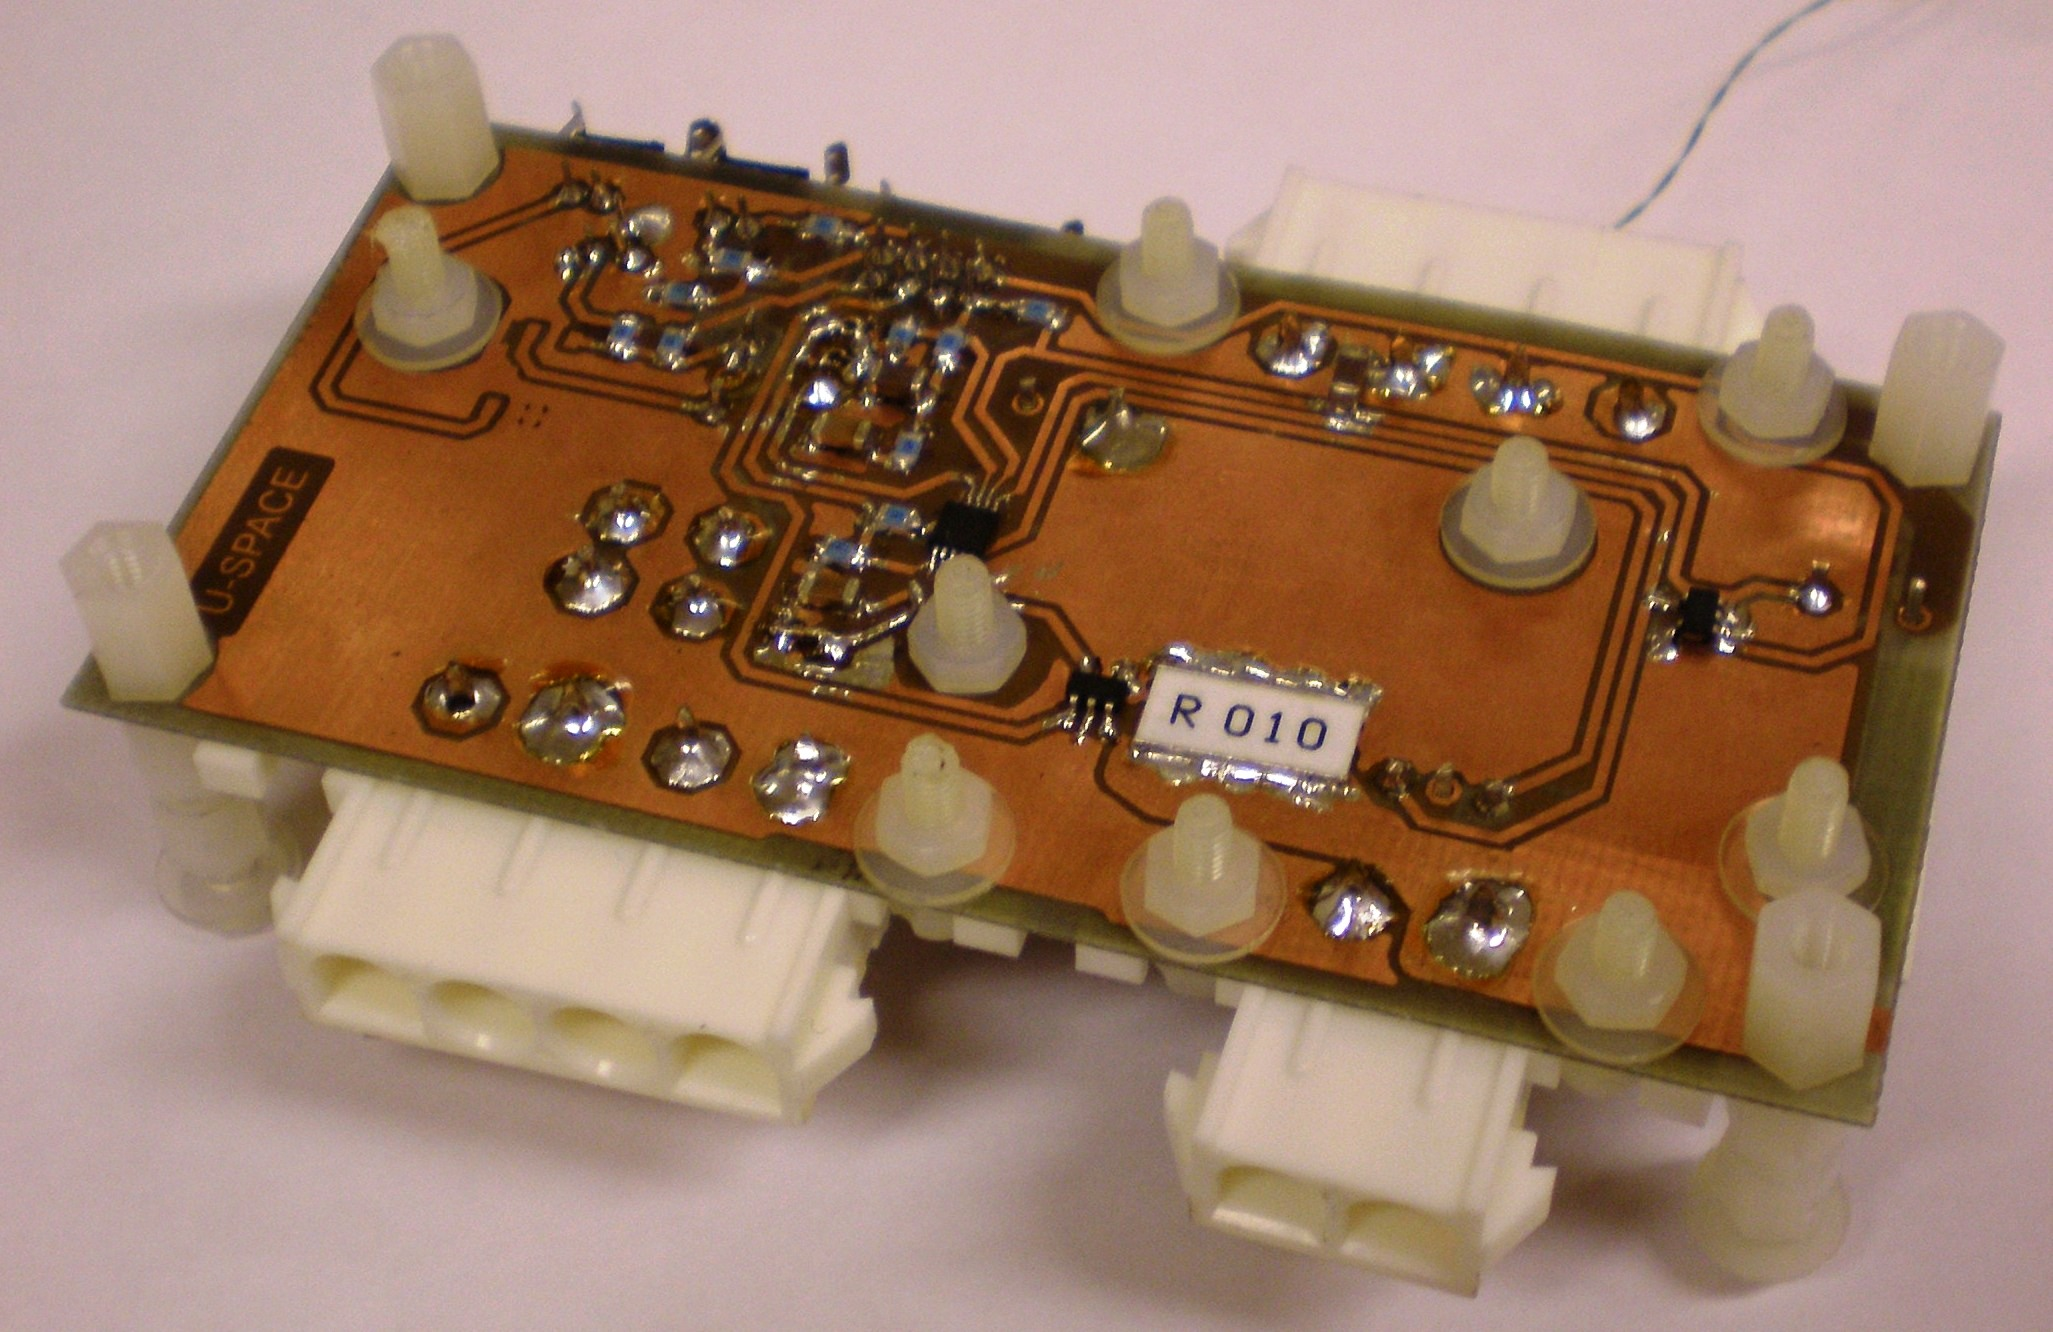
\includegraphics[width=0.7\textwidth]{figures/fig_BCR_bottom}
\end{minipage}
\caption{Battery Charge Regulator}
\label{fig:BCR_top_bottom}
\end{figure}
%
\begin{figure}[H]
\centering
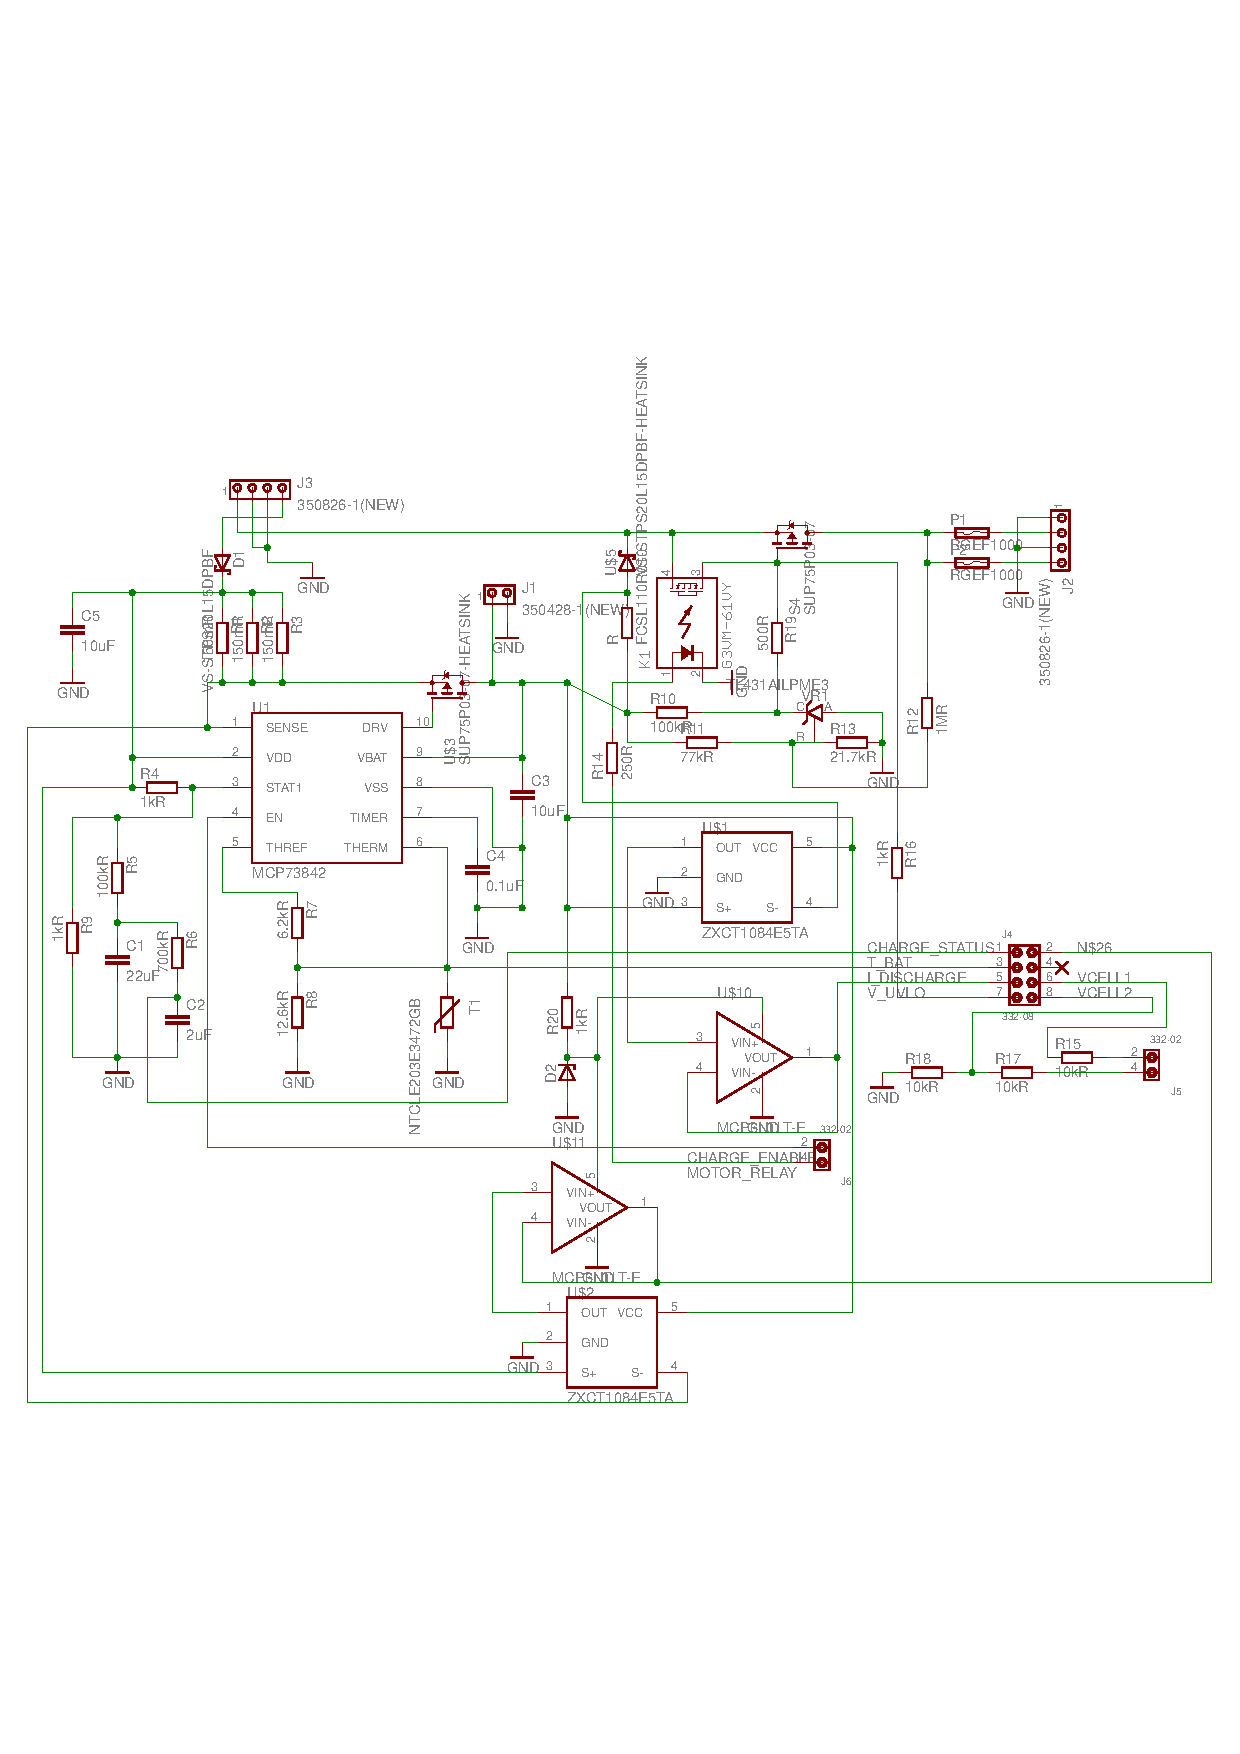
\includegraphics[width=\textwidth]{figures/fig_Schematic_BCR}
\caption{Schematic of the \acl{BCR}}
\label{fig:BCR_Schematic}
\end{figure}
%
%
\subsection{Solar Array Regulator}

5.0V(regulated), 3.3V(regulated),

Inclusion of 3.3V regulated output - mainly due to limitations on BeagleBoard which is not compatible with 5V?

SAR not implemented due to time limitation.

MPPT not implemented due to time limitation.

Components for DC-DC converter already ordered.

Additional telemetry data outputs added for SAR.

\begin{figure}[H]
\begin{minipage}[t]{\linewidth}
\centering
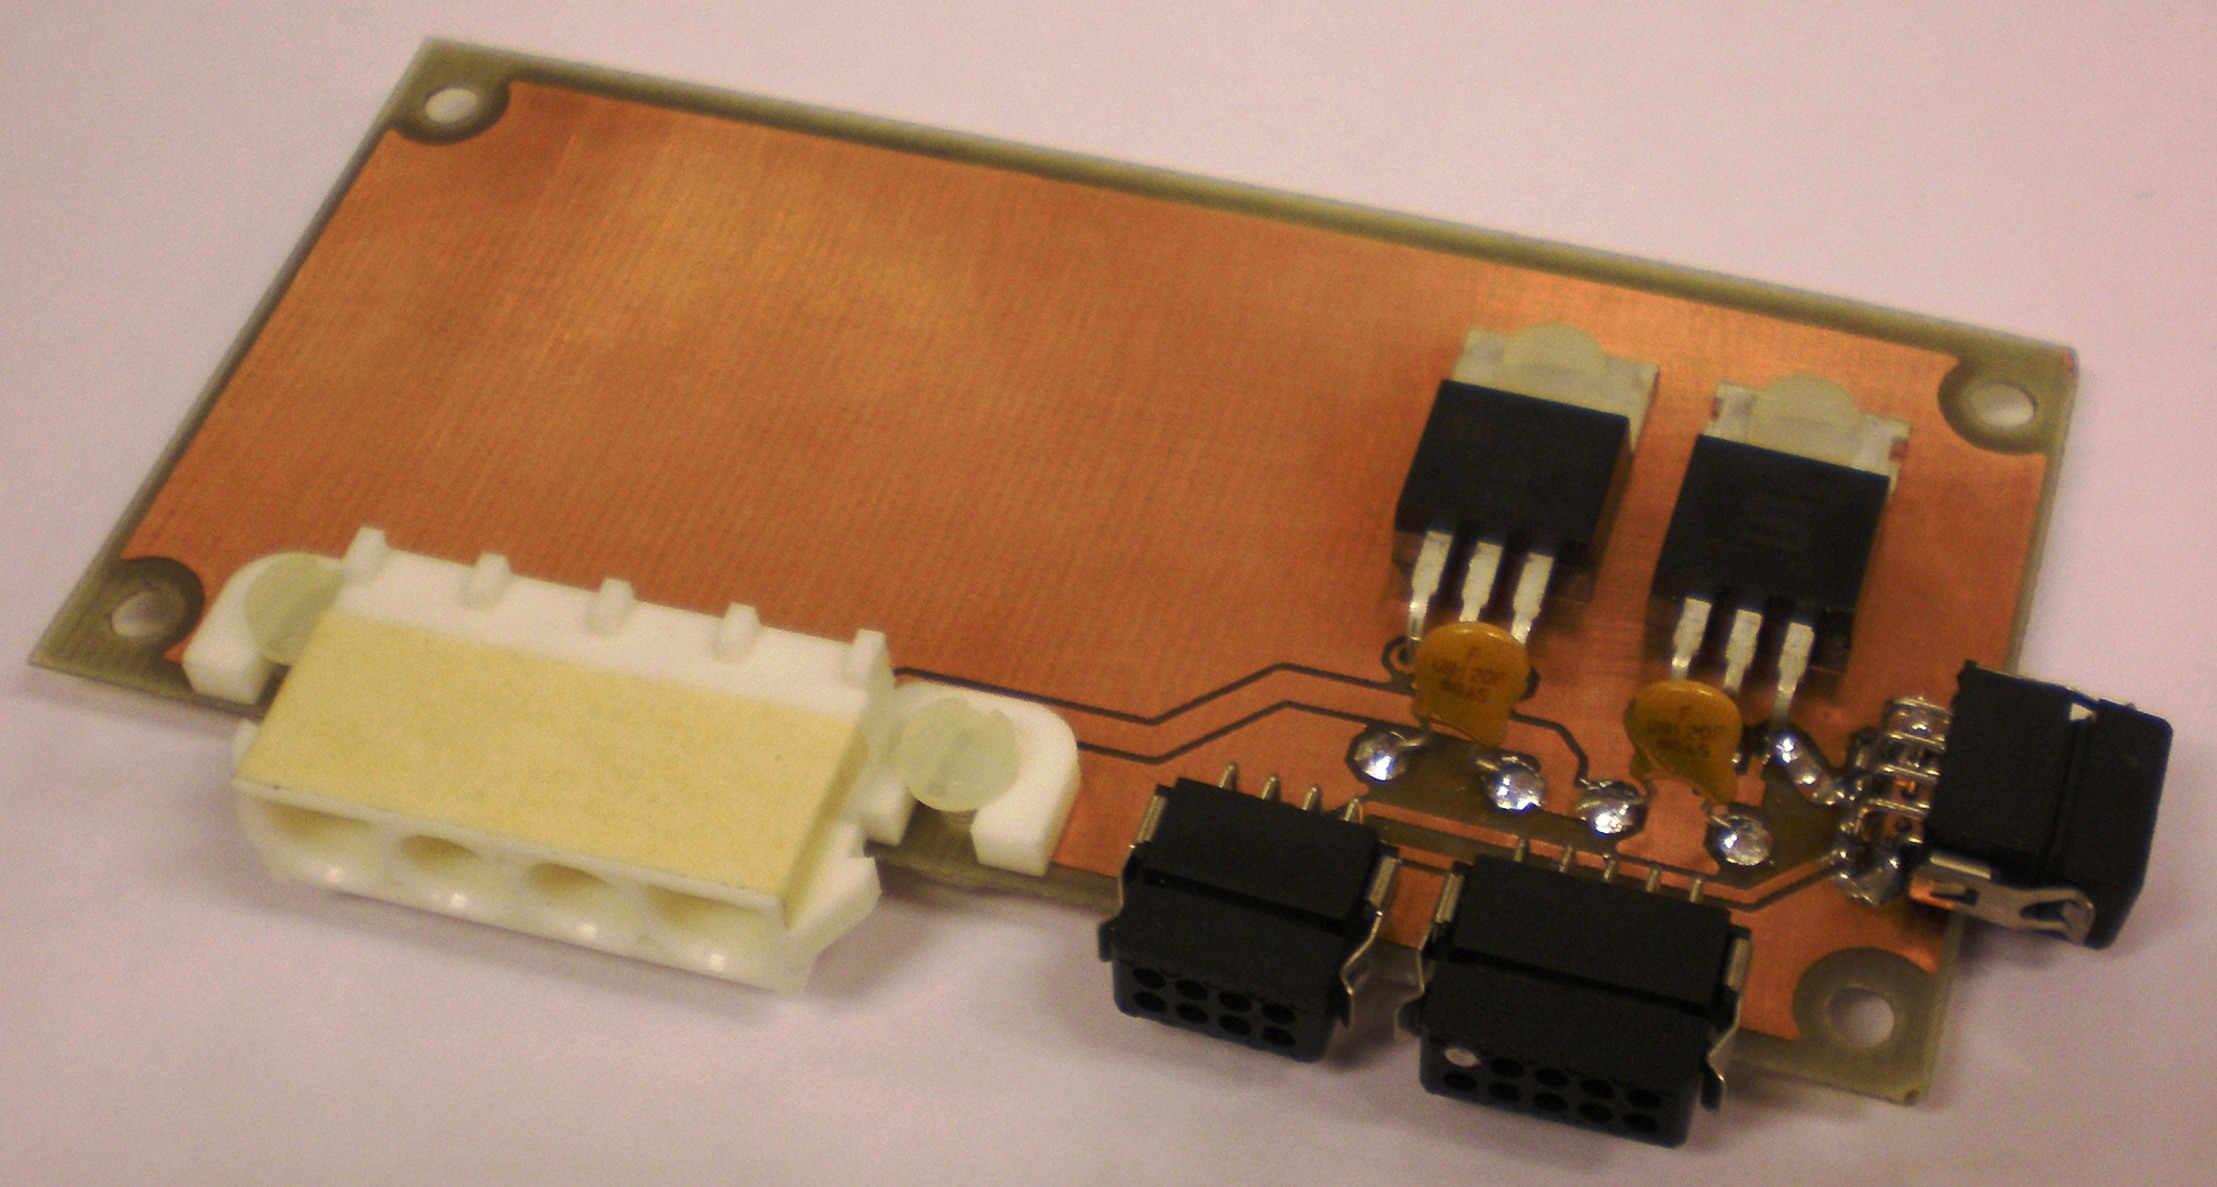
\includegraphics[width=0.7\textwidth]{figures/fig_SAR_top}
\end{minipage}
\vspace{2mm}
\begin{minipage}[t]{\linewidth}
\centering
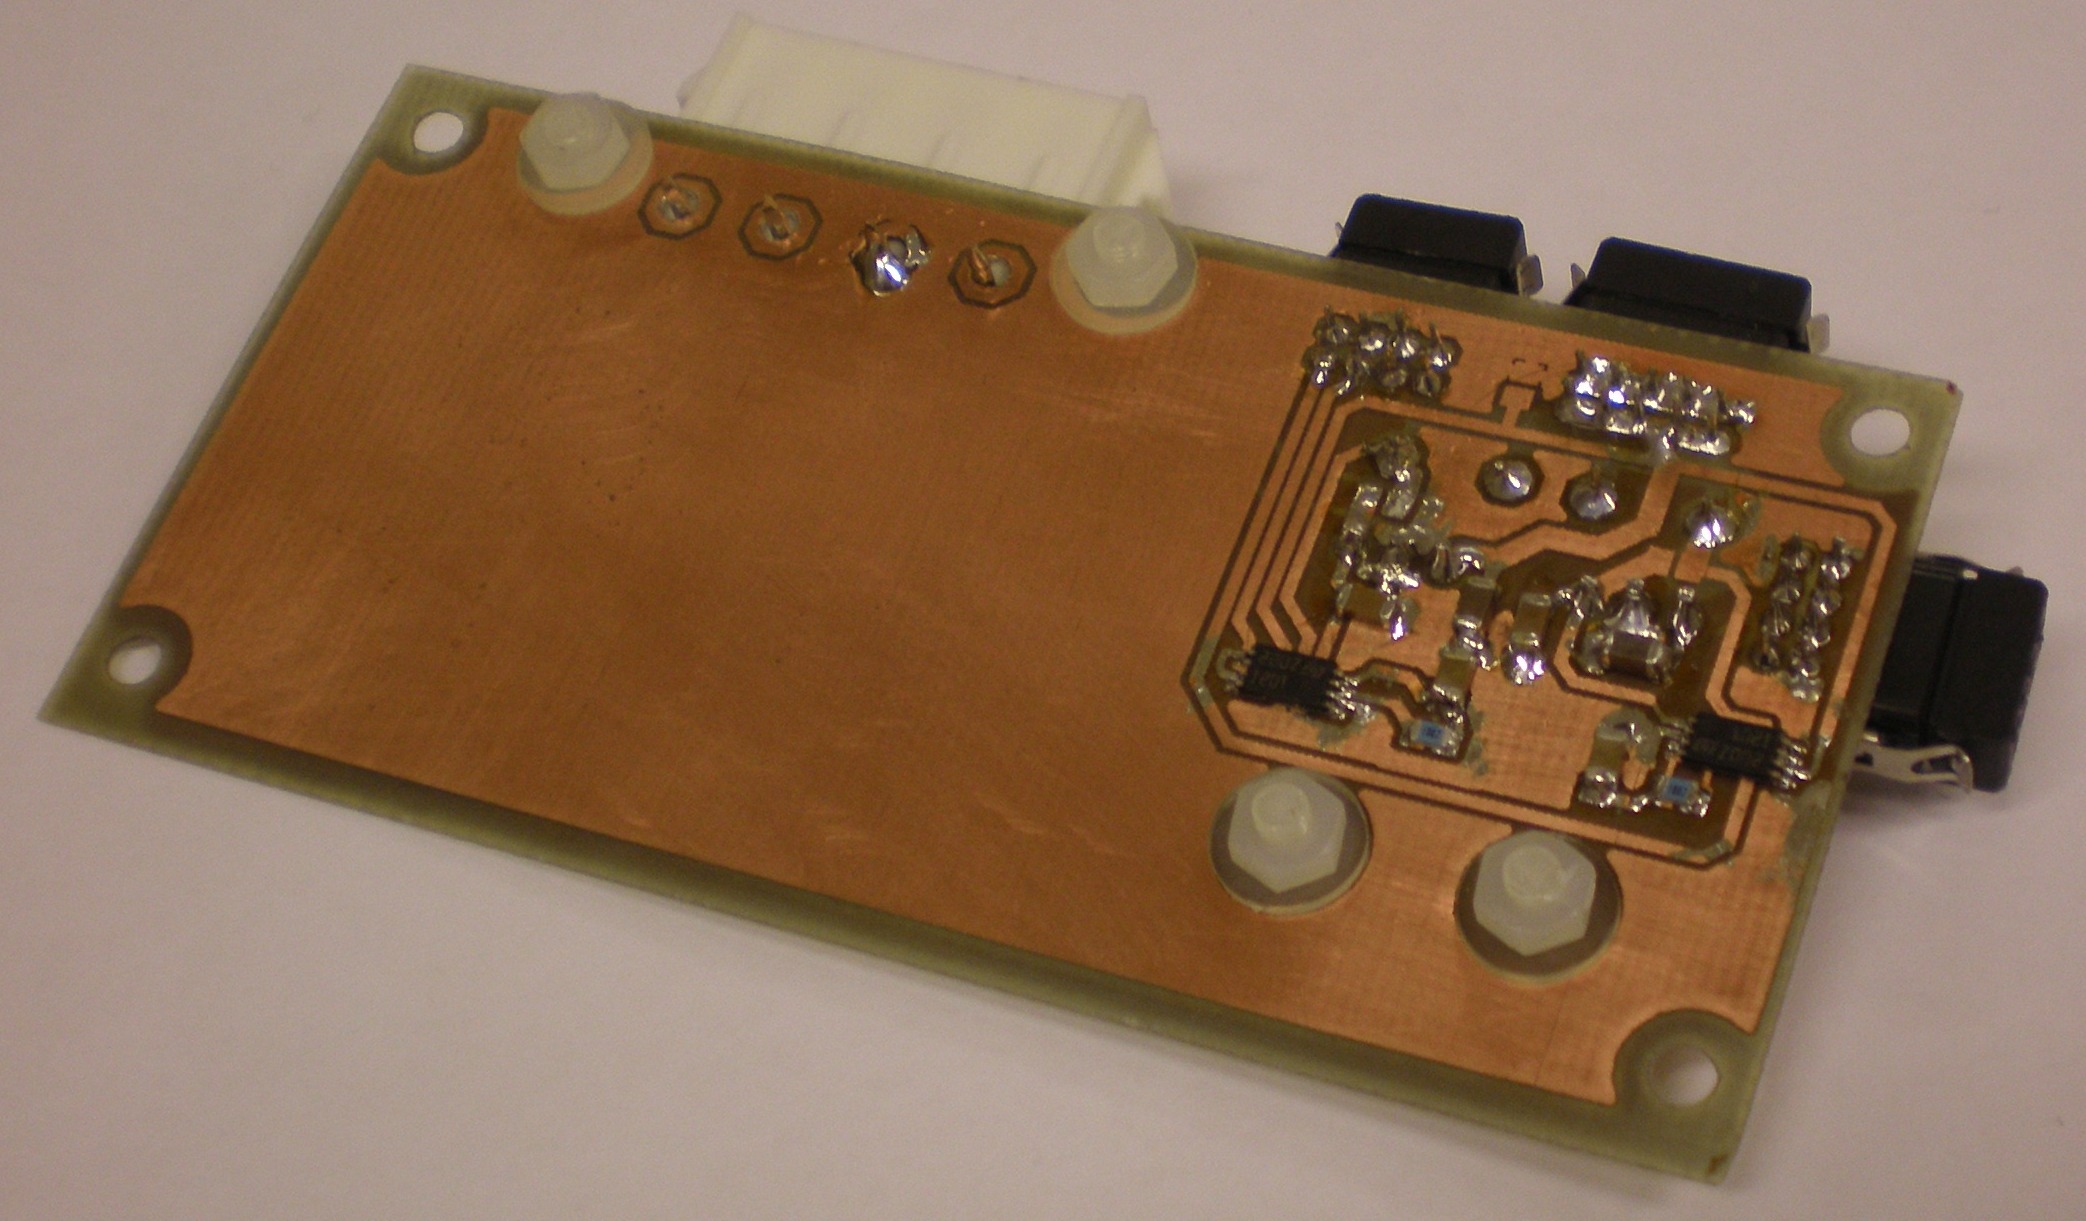
\includegraphics[width=0.7\textwidth]{figures/fig_SAR_bottom}
\end{minipage}
\caption{Battery Charge Regulator}
\label{fig:SAR_top_bottom}
\end{figure}

\begin{figure}[H]
\centering
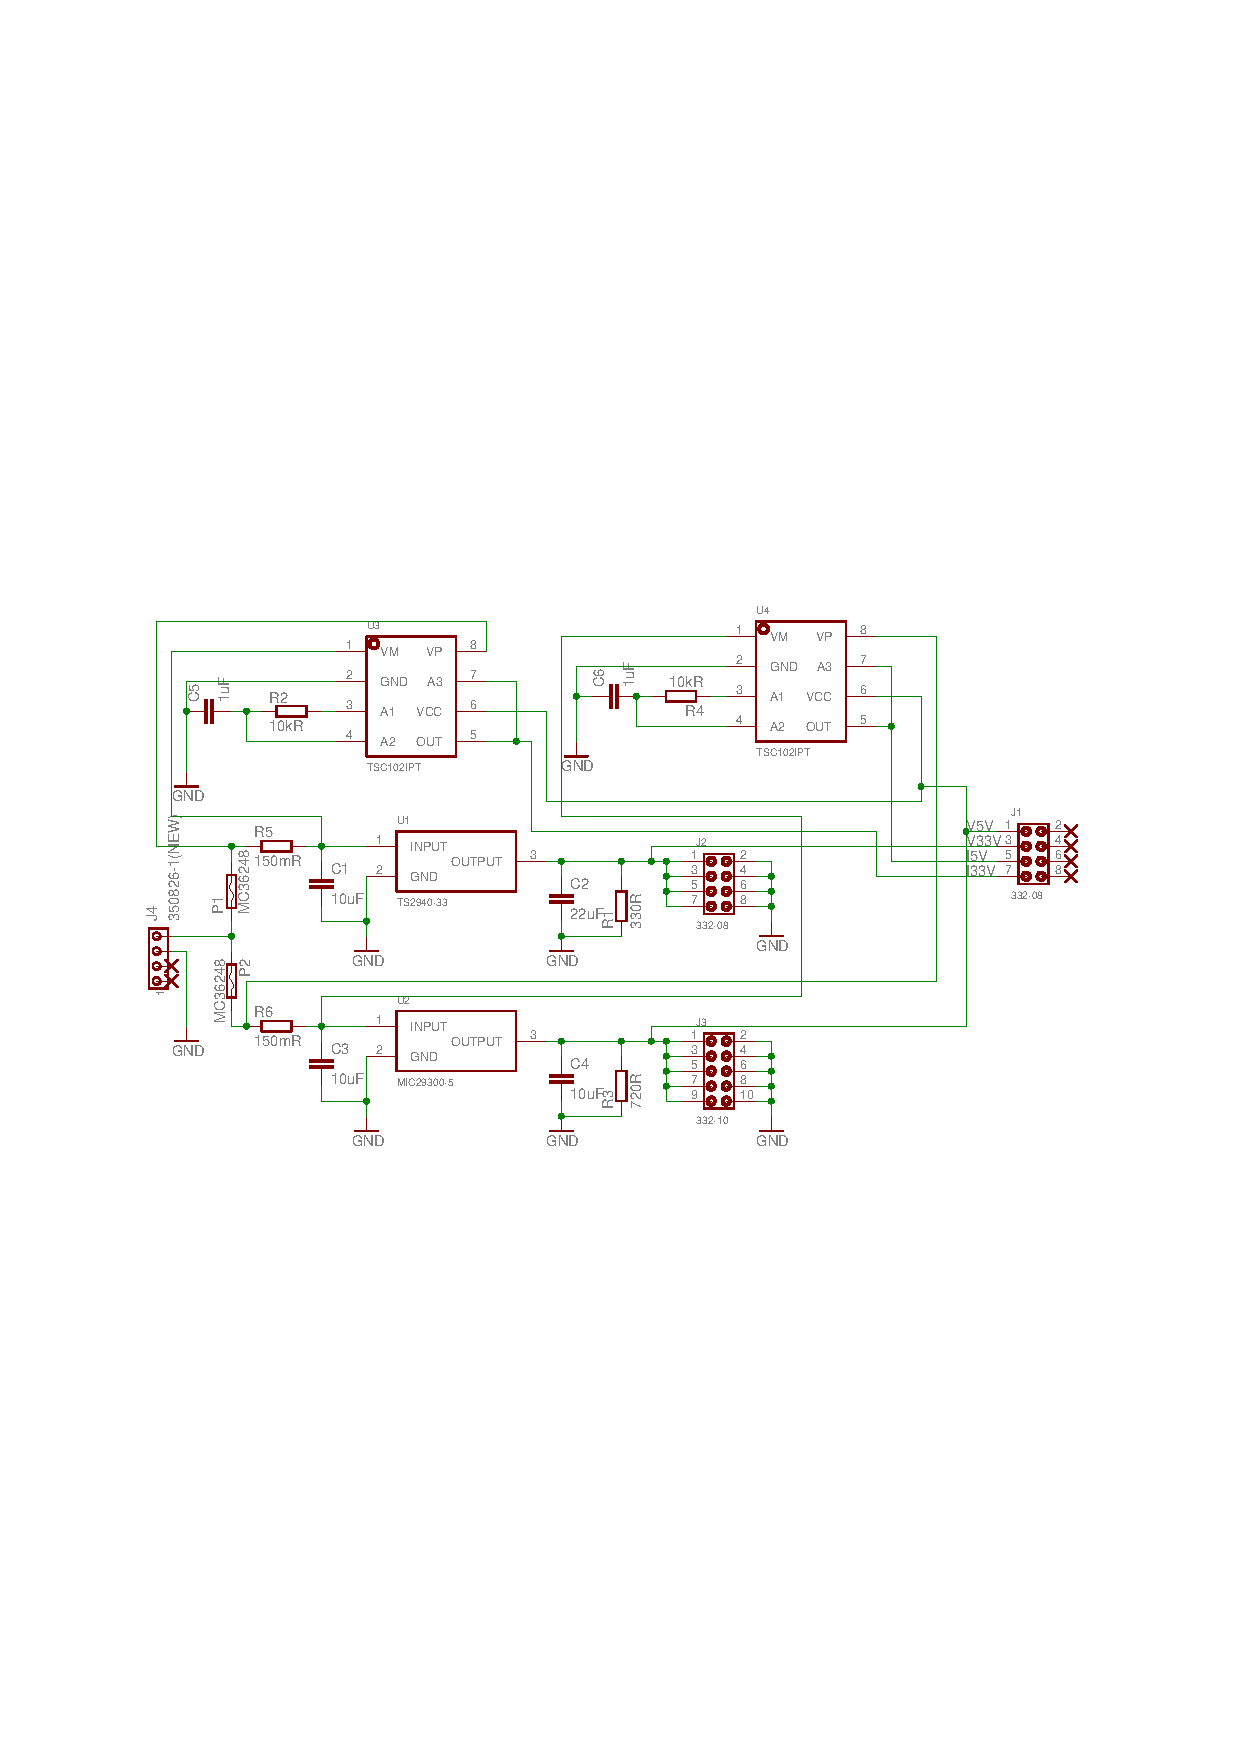
\includegraphics[width=\textwidth]{figures/fig_Schematic_SAR}
\caption{Schematic of the \acl{SAR}}
\label{fig:SAR_Schematic}
\end{figure}


\subsection{Temperature Sensor Board}


\begin{figure}[H]
\centering
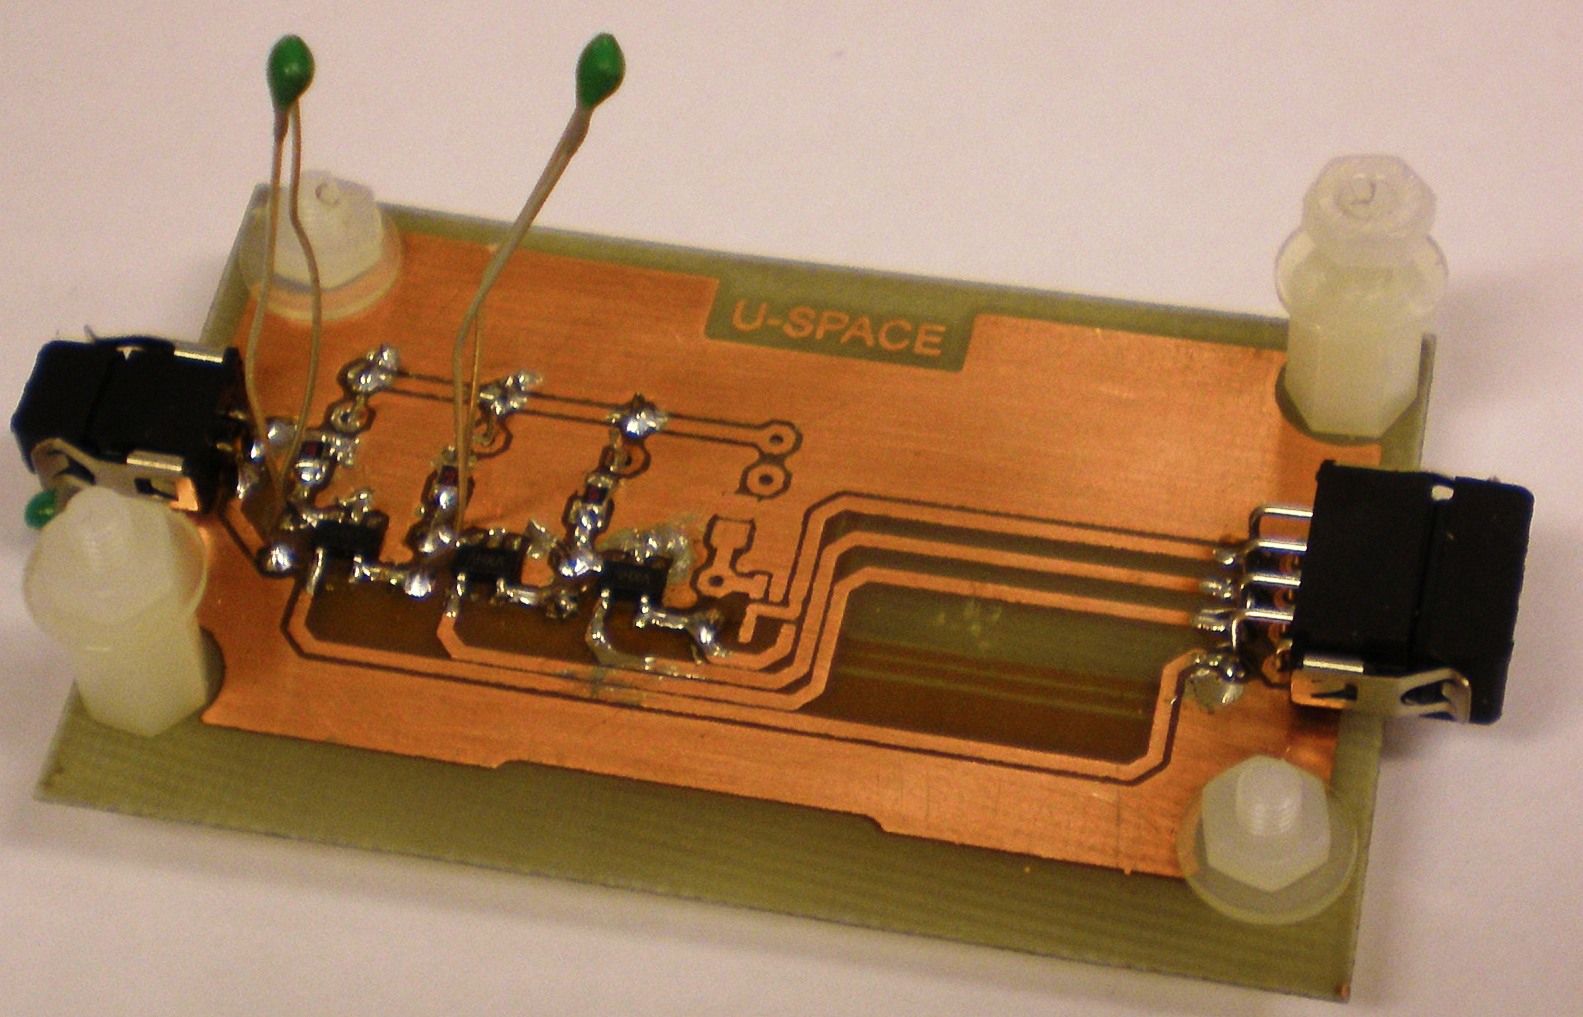
\includegraphics[width=0.7\textwidth]{figures/fig_Temp_top}
\caption{Temperature Sensor Board}
\label{fig:TS_top}
\end{figure}

\begin{figure}[H]
\centering
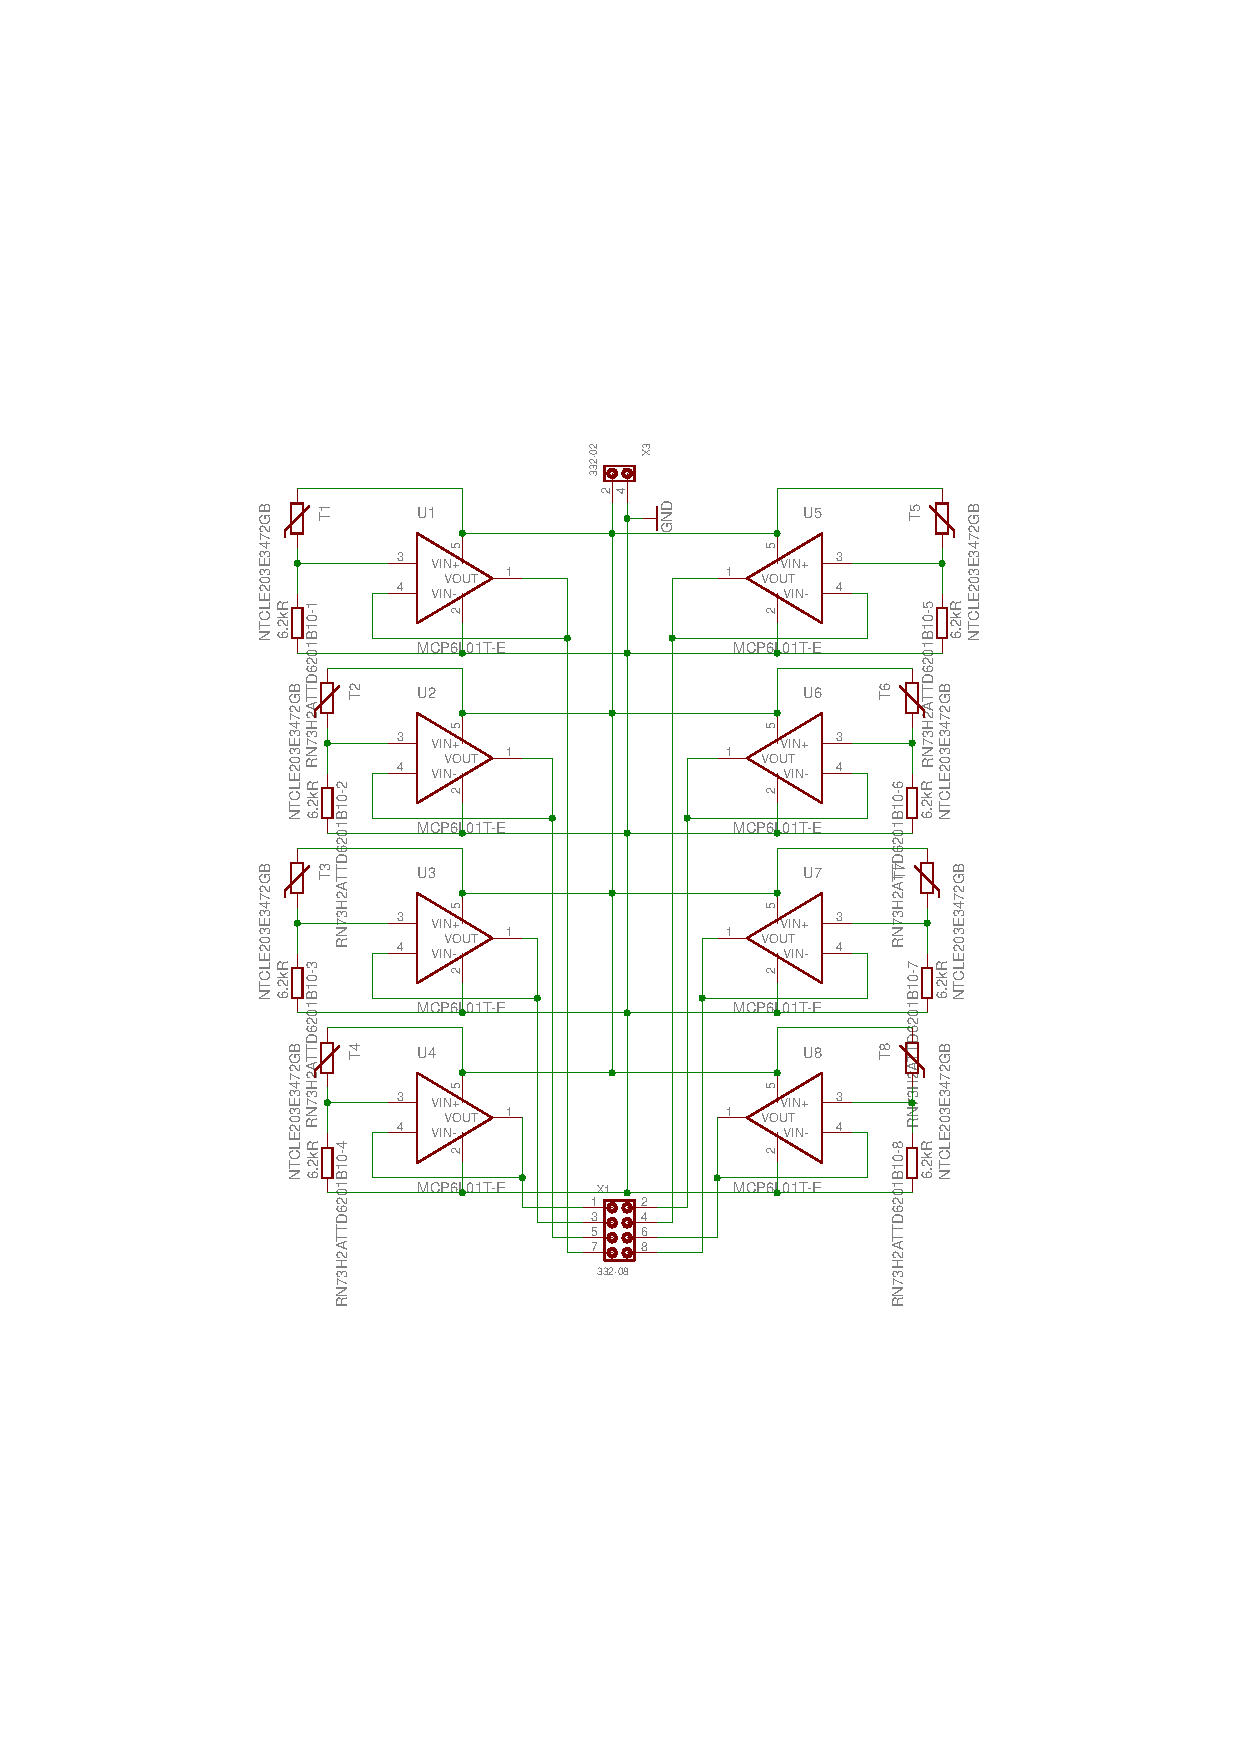
\includegraphics[width=\textwidth]{figures/fig_Schematic_TS}
\caption{Schematic of the Temperature Sensor Board}
\label{fig:Schematic_TS}
\end{figure}


\section{Mechanical Structure and Envelope}
%responsible: Pedro 

\section{Motor Control and Communication}
%responsible: Pedro and Morten

Temperature monitoring not implemented due to lack of thin wire (ordered thin wire proved to be non-practical to work with = too fragile).


\section{Imaging and Tracking Payload Unit}
%responsible: Jan

\section{Telecommunication}
%responsible: Omair